\documentclass[xcolor={usenames,dvipsnames,svgnames}]{beamer}
\usetheme{/sesarbeamer}

\usepackage{cite}

\usepackage{adjustbox}
\usepackage[acronym]{glossaries}
% \usepackage{xcolor}

% \newacronym{API}{API}{Application Programming Interface}
% \newacronym{CA}{CA}{Certification Agent}
% \newacronym{CDN}{CDN}{Content Distribution Network}
% \newacronym{CLI}{CLI}{Command Line Interface}
% \newacronym{CSV}{CSV}{Comma Separated Values}
% \newacronym{DAG}{DAG}{Directed Acyclic Graph}
% \newacronym{DNS}{DNS}{Domain Name System}
% \newacronym{FIFO}{FIFO}{First In First Out}
% \newacronym{GLB}{GLB}{Greatest Lower Bound}
% \newacronym{HTTP}{HTTP}{HyperText Transfer Protocol}
% \newacronym{HTTPS}{HTTPS}{HyperText Transfer Protocol over Secure Socket Layer}
% \newacronym{ISP}{ISP}{Internet Service Provider}
% \newacronym{IXP}{IXP}{Internet Exchange Point}
% \newacronym{LRU}{LRU}{Least Recently Used}
% \newacronym{LUB}{LUB}{Least Upper Bound}
% \newacronym{PIT}{PIT}{Pending Interest Table}
\newacronym{QoS}{QoS}{Quality of Service}
% \newacronym{RTT}{RTT}{Round Trip Time}
% \newacronym{TCP}{TCP}{Transmission Control Protocol}
% \newacronym{TLS}{TLS}{Transport Layer Security}
% \newacronym{URI}{URI}{Uniform Resource Identifier}
\newacronym{KPI}{KPI}{Key Performance Indicator}

% 5G system components
\newacronym{AF}{AF}{Application Function}
\newacronym{AM}{AM}{Access and Mobility Function}
\newacronym{AMF}{AMF}{Access and mobility Management Function}
\newacronym{AUSF}{AUSF}{Authentication Server Function}
\newacronym{CP}{CP}{Control Plane}
\newacronym{CPF}{CPF}{Control Plane Function}
\newacronym{NEF}{NEF}{Network Exposure Function}
\newacronym{NF}{NF}{Network Function}
\newacronym{NRF}{NRF}{Network Repository Function}
\newacronym{NSSAI}{NSSAI}{Network Slice Selection Assistance Information}
\newacronym{NSSF}{NSSF}{Network Slice Selection Function}
\newacronym{NSS}{NSS}{Network Slice Selection Function}
\newacronym{PCF}{PCF}{Policy Control Function}
\newacronym{SCP}{SCP}{Service Communication Proxy}
\newacronym{SMF}{SMF}{Session Management Function}
\newacronym{UDM}{UDM}{Unified Data Management}
\newacronym{UDR}{UDR}{Unified Data Repository}
\newacronym{UE}{UE}{User Equipment}
\newacronym{UPF}{UPF}{User Plane Function}
\newacronym{UP}{UP}{User Plane}

\newacronym{CSMF}{CSMF}{Communication Service Management Function}
\newacronym{EAP}{EAP}{Extensible Authentication Protocol}
\newacronym{MEAO}{MEAO}{Mobile Edge Application Orchestrator}
\newacronym{MEC}{MEC}{Multi-access Edge Computing}
\newacronym{MEP}{MEP}{Mobile Edge Platform}
\newacronym{MEPM}{MEPM}{Mobile Edge Platform Manager}
\newacronym{NSSMF}{NSSMF}{Network Slice Subnet Management Function}
\newacronym{RCS}{RCS}{Rich Communication Services}
\newacronym{SLA}{SLA}{Service Level Agreement}
\newacronym{SLO}{SLO}{Service Level Objective}
\newacronym{VIM}{VIM}{Virtualization Infrastructure Manager}
\newacronym{VNFD}{VNFD}{Virtualized Network Function Descriptor}
\newacronym{VNFO}{VNFO}{Virtualized Network Function Orchestrator}
\newacronym{VNF}{VNF}{Virtualized Network Function}


\usepackage{tikz}
\usetikzlibrary{
	calc,
	arrows.meta,
	backgrounds,
	calc,
	fit,
	positioning,
	shadows,
	shapes.arrows,
	shapes.geometric,
	shapes.symbols
}

\newcommand{\inputtikz}[1]{%
	\tikzsetnextfilename{#1}%
	\input{#1}%
}

\tikzset{%
	base/.style = {
			% minimum width=1cm, 
			% minimum height=1cm, 
			text centered,
			% font=\sffamily,
			inner sep=0.5em,
		},
	boxes/.style = {
			base,
			draw=black,
			rectangle,
			rounded corners
		},
	arrow_label/.style = {
			base,
			midway,
			% sloped,
			fill=white, anchor=center,
		},
	on slide/.code args={<#1>#2}{%
			\only<#1>{\pgfkeysalso{#2}}%
		},
}


% meta-data
\title{Intent-based management of 5G infrastructures}
\subtitle{Future research topics}
\author{\href{mailto:filippo.berto@unimi.it}{Filippo Berto}}
\date{May 5th, 2023}
% \titlebackground{images/background}

% document body
\begin{document}

\maketitle

\section{Intent based infrastructure management}

\begin{frame}{Infrastructure adaptation}
	\begin{columns}
		\begin{column}{.4\textwidth}
			Telco and edge computing infrastructure are \alert{complex} and their configuration is a \alert{costly} and \alert{error-prone} task. \vspace{1em}

			We want the infrastructure to \alert{update automatically} and \alert{optimally} based on environmental changes.
		\end{column}
		\begin{column}<2->{.5\textwidth}
			Optimizing
			\begin{itemize}
				\item resources utilization (network, computation, external services, \ldots)
				\item services deployment (location, traffic, resources, \ldots)
			\end{itemize}
			for \alert{minimizing costs} while meeting \alert{\glspl{SLA}}.\vspace{1em}

			Resource allocation and configuration is \alert{negotiated} between the parties.
		\end{column}
	\end{columns}
\end{frame}

\begin{frame}{Intent based configuration}
	\begin{columns}
		\begin{column}{.5\textwidth}
			We build an \alert{abstract model} of the system with:
			\begin{itemize}
				\item a set of \alert{rules} (functional requirements, \glspl{SLA}, \ldots)
				\item \alert{inputs} (status measurements, configuration intents)
				\item \alert{outputs} (new configurations)
				\item a \alert{goal} (i.e.\ cost minimization).
			\end{itemize}
		\end{column}
		\begin{column}<2->{.5\textwidth}
			\alert{Itents} are prescriptions used to propose changes, like services deployments or network changes. \vspace{1em}

			\alert{Monitoring} cyclically produces new measurements of the system state \vspace{1em}

			When new inputs are provided, the model checks for \alert{feasibility} and produces a new \alert{optimal configuration}.
		\end{column}
	\end{columns}
\end{frame}

% \section{Research topics}

% \begin{frame}{5G core network}
% 	\vfill
% 	\begin{adjustbox}{max totalsize={0.9\linewidth}{\textheight},center}
% 		\begin{tikzpicture}[align=center, auto, style={base}]
	\begin{scope}[every node/.style={boxes, fill=Grey!10}]
		\node (nssf) [] {\acrshort*{NSSF}\\\scriptsize\acrlong*{NSSF}};
		\node (nef) [right = 0.5 of nssf] {\acrshort*{NEF}\\\scriptsize\acrlong*{NEF}};
		\node (nrf) [right = 0.5 of nef]{\acrshort*{NRF}\\\scriptsize\acrlong*{NRF}};
		\node (pcf) [right = 0.5 of nrf]{\acrshort*{PCF}\\\scriptsize\acrlong*{PCF}};
		\node (ausf) at ($(nssf) + (-0.5,-2)$) [] {\acrshort*{AUSF}\\\scriptsize\acrlong*{AUSF}};
		\node (amf) [right = 0.5 of ausf] {\acrshort*{AMF}\\\scriptsize\acrlong*{AMF}};
		\node (smf) [right = 0.5 of amf] {\acrshort*{SMF}\\\scriptsize\acrlong*{SMF}};
		\node (udm) [right = 0.5 of smf]{\acrshort*{UDM}\\\scriptsize\acrlong*{UDM}};
		\uncover<2->{\node (other_nf) [right = 0.5 of udm] {Other \acrshort*{NF}s};}
		\uncover<2->{\node (mec1) [right = 0.5 of pcf, fill=Orange!50] {\acrshort*{MEC}};}
		\uncover<2->{\node (mec2) [right = 0.5 of mec1, fill=Orange!50] {\acrshort*{MEC}};}
		\uncover<2->{\node (mec3) [right = 0.5 of mec2, fill=Orange!50] {\acrshort*{MEC}};}
		\node (ran) [below = 1 of amf] {\acrshort*{RAN}\\\scriptsize\acrlong*{RAN}};
		\node (ue) [left = 3 of ran, fill=OrangeRed!25] {\acrshort*{UE}\\\scriptsize\acrlong*{UE}};
		\node (upf) [below = 1 of smf] {\acrshort*{UPF}\\\scriptsize\acrlong*{UPF}};
	\end{scope}
	\node (ladn) [
		right = 4 of upf,
		cloud,
		aspect=2,
		cloud puffs=13.7,
		fill=YellowGreen!50,
		inner sep=-0.5em,
		draw
	] {\acrshort*{LADN}\\\scriptsize\acrlong*{LADN}};

	\only<1>{\draw [very thick] ($(ausf) + (-0.5,1)$) to ($(udm) + (0.5,1)$)};
	\only<2->{\draw [very thick] ($(ausf) + (-0.5,1)$) to ($(mec3) + (0.5,-1)$)};
	\foreach \i in {nssf,nef,nrf,pcf}{\draw [-Circle](\i) to ($(\i) + (0,-1.06)$);}
	\foreach \i in {ausf,amf,smf,udm}{\draw [-Circle] (\i) to ($(\i) + (0,1.06)$);}
	\uncover<2->{\foreach \i in {mec1,mec2,mec3}{\draw [-Circle](\i) to ($(\i) + (0,-1.06)$);}}
	\uncover<2->{\foreach \i in {other_nf}{\draw [-Circle] (\i) to ($(\i) + (0,1.06)$);}}
	\draw (ue) -- (amf) node [midway,fill=white,sloped,anchor=center] {N1};
	\draw (ran) -- (amf) node [midway,fill=white,anchor=center] {N2};
	\draw (ran) -- (upf) node [midway,fill=white,anchor=center] {N3};
	\draw (upf) -- (ladn) node [midway,fill=white,anchor=center] {N6};
	\draw (upf) -- (smf) node [midway,fill=white,anchor=center] {N4};
	\draw (ue) to (ran);
\end{tikzpicture}

% 	\end{adjustbox}
% 	\begin{columns}[T]
% 		\begin{column}{.5\textwidth}
% 			\begin{itemize}
% 				\item<1-> Infrastructure as composition of microservices and hardware
% 				\item<1-> Transparent API for interchangeable components implementations
% 			\end{itemize}
% 		\end{column}
% 		\begin{column}{.5\textwidth}
% 			\begin{itemize}
% 				\item<2-> Deployment of services as Network Functions in the Core Network MEC
% 				\item<2-> 5G network infrastructure nodes as a layer in the edge cloud continuum
% 			\end{itemize}
% 		\end{column}
% 	\end{columns}
% 	\vfill
% \end{frame}

% \begin{frame}{O-RAN architecture}
% 	\vfill
% 	\begin{columns}
% 		\begin{column}{.45\textwidth}
% 			\begin{itemize}
% 				\item Standardization of RAN components implementations
% 				\item RAN Intelligent Controller controls and optimizes the available resources
% 				\item Central and Distributed units handle resources and lower network layers
% 				\item Radio Unit manages the radio physical layer
% 				\item O-Cloud provides a standardized cloud platform hosting network functions
% 			\end{itemize}
% 		\end{column}
% 		\begin{column}{.55\textwidth}
% 			\centering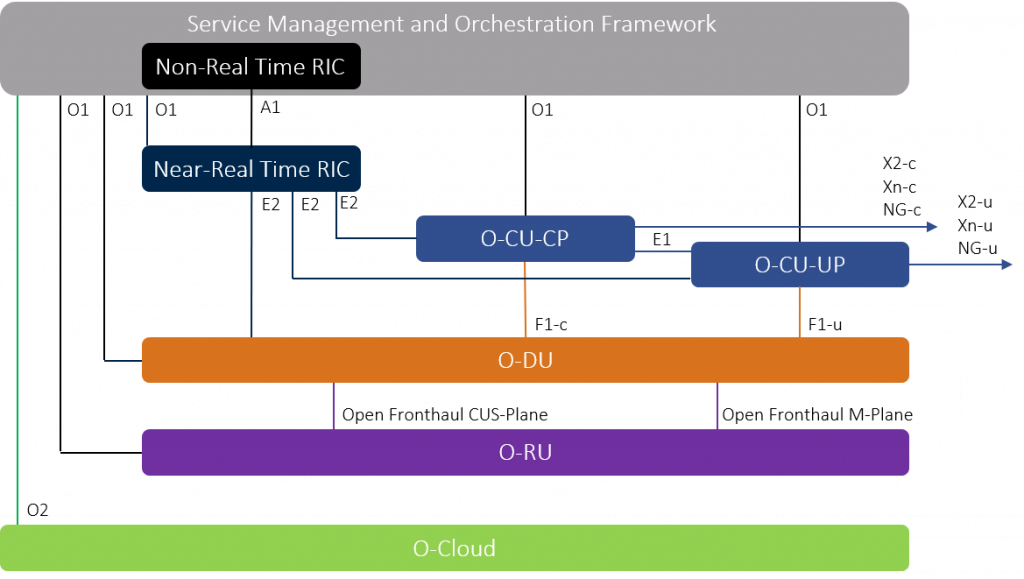
\includegraphics[width=\textwidth]{images/oran.png}
% 		\end{column}
% 	\end{columns}
% 	\vfill
% \end{frame}

\section{Objectives}

\begin{frame}{Research objectives}
	\begin{itemize}
		\setlength\itemsep{1em}
		\item Transparent infrastructure \gls{QoS} monitoring framework
		\item Extensible intent format definition
		\item Implementation of an adaptation framework for the 5G network
		\item Integration of the framework with state-of-the-art technologies (O-RAN, Open Source MANO, Kubernetes)
	\end{itemize}
\end{frame}

\section{Expected results and benefits}

\begin{frame}{Expected results}
	\begin{itemize}
		\setlength\itemsep{1em}
		\item Improved transparency of infrastructure and services deployed on the edge
		\item Intent based network configuration of the network
		\item \gls{QoS} requirements aware deployment infrastructure and resource management
		\item Development of a framework to extend deployment compositions
	\end{itemize}
\end{frame}

\begin{frame}{Expected benefits}
	\begin{itemize}
		\setlength\itemsep{1em}
		\item Development of the O-RAN and OSM infrastructure, in use by the TMF Catalyst Project ``IDAN Phase III'' (which University of Milan and TIM are part of)
		\item TIM can adopt part of the framework, improving its infrastructure efficiency and providing its users with transparent \gls{QoS} evidence
		\item Results can be reused in the infrastructure of PNRR  Project ``MUSA''
		\item Integration of the solution in a real world test bed drives us to raise the solution's readiness level.
	\end{itemize}
\end{frame}

\begin{frame}[allowframebreaks]{References}{~}
	\nocite{
		anisetti2022security,
		anisetti2022assurance,
		anisetti2022orchestration,
		anisetti2022devsecops,
		berto20225g,
		anisetti2021security,
		berto2020spatial
	}
	\bibliographystyle{IEEEtran}\small
	\bibliography{biblio.bib}
\end{frame}
% \begin{frame}

% 	This template is a secondary creation of SESAR Presentation template from \hrefcol{mailto:filippo.berto@unimi.it}{Filippo Berto} \vspace{2baselineskip}

% 	Following is a brief introduction written by \hrefcol{mailto:filippo.berto@unimi.it}{Filippo Berto} about how to use \LaTeX\ and beamer to prepare slides. All rights reserved by him\vspace{2baselineskip}

% 	This template is released under \hrefcol{https://creativecommons.org/licenses/by-nc/4.0/legalcode}{Creative Commons CC BY 4.0} license

% \end{frame}

% \section{Introduction}

% \begin{frame}{Beamer for SESAR slides}{\thesection \, \secname}

% 	\begin{itemize}
% 		\item We assume you can use \LaTeX; if you cannot,
% 		      \hrefcol{http://en.wikibooks.org/wiki/LaTeX/}{you can learn it here}
% 		\item Beamer is one of the most popular and powerful document
% 		      classes for presentations in \LaTeX
% 		\item Beamer has also a detailed
% 		      \hrefcol{http://www.ctan.org/tex-archive/macros/latex/contrib/beamer/doc/beameruserguide.pdf}{user manual}
% 		\item Here we will present only the most basic features to get you up to speed
% 	\end{itemize}
% \end{frame}

% \begin{frame}{Beamer vs. PowerPoint}
% 	Compared to PowerPoint, using \LaTeX\ is better because:
% 	\begin{itemize}
% 		\item It is not What-You-See-Is-What-You-Get, but
% 		      What-You-\emph{Mean}-Is-What-You-Get:\\
% 		      you write the content, the computer does the typesetting
% 		\item Produces a \texttt{pdf}: no problems with fonts, formulas,
% 		      program versions
% 		\item Easier to keep consistent style, fonts, highlighting, etc.
% 		\item Math typesetting in \TeX\ is the best:
% 		      \begin{equation*}
% 			      \mathrm{i}\,\hslash\frac{\partial}{\partial t} \Psi(\mathbf{r},t) =
% 			      -\frac{\hslash^2}{2\,m}\nabla^2\Psi(\mathbf{r},t)
% 			      + V(\mathbf{r})\Psi(\mathbf{r},t)
% 		      \end{equation*}

% 	\end{itemize}
% \end{frame}

% \section{Editing}

% \begin{frame}[fragile]{Selecting the Class}
% 	To start working with \texttt{SESARbeamer}, start a \LaTeX\ document with the
% 	preamble:
% 	\begin{block}{Minimum SESAR Beamer Document}
% 		\begin{lstlisting}[language=TeX]
% \documentclass{beamer}
% \usetheme{/sesarbeamer}
% \begin{document}
% \begin{frame}{Hello, world!}
% \end {frame}
% \end{document}
% \end{lstlisting}
% 	\end{block}
% \end{frame}

% \begin{frame}[fragile]{Title page}
% 	To set a typical title page, you call some commands in the preamble:
% 	\begin{block}{The Commands for the Title Page}
% 		\begin{lstlisting}[language=TeX]
% \title{Sample Title}
% \subtitle{Sample subtitle}
% \author{First Author, Second Author}
% \date{Defaults to today's}
% \end{lstlisting}
% 	\end{block}
% 	You can then write out the title page with \verb|\maketitle|.

% 	You can set a different background image than the default one with the
% 	\verb|\titlebackground| command, set before \verb|\maketitle|.

% 	In the \texttt{backgrounds} folder, you can find a lot of standard backgrounds
% 	for SESAR presentation title pages.

% \end{frame}

% \begin{frame}[fragile]{Writing a Simple Slide}
% 	\framesubtitle{It's really easy!}
% 	\begin{itemize}[<+->]
% 		\item A typical slide has bulleted lists
% 		\item These can be uncovered in sequence
% 	\end{itemize}
% 	\begin{block}{Code for a Page with an Itemised List}<+->
% 		\begin{lstlisting}[language=TeX]
% \begin{frame}
%   \frametitle{Writing a Simple Slide}
%   \framesubtitle{It's really easy!}
%   \begin{itemize}[<+->]
%     \item A typical slide has bulleted lists
%     \item These can be uncovered in sequence
%   \end{itemize}
% \end{frame}\end{lstlisting}
% 	\end{block}
% \end{frame}

% \begin{frame}[fragile]{Adding images}
% 	\begin{columns}
% 		\begin{column}{0.7\textwidth}
% 			Adding images works like in normal \LaTeX:
% 			\begin{block}{Code for Adding Images}
% 				\begin{lstlisting}[language=TeX]
% \usepackage{graphicx}
% % ...
% \includegraphics
% [width=\textwidth]{images/default}
% \end{lstlisting}
% 			\end{block}
% 		\end{column}
% 		\begin{column}{0.3\textwidth}
% 			\includegraphics
% 			[width=\textwidth]{images/default}\\
% 		\end{column}
% 	\end{columns}
% \end{frame}

% \begin{frame}[fragile]{Splitting in Columns}
% 	Splitting the page is easy and common;
% 	typically, one side has a picture and the other text:
% 	\begin{columns}
% 		\begin{column}{0.6\textwidth}
% 			This is the first column
% 		\end{column}
% 		\begin{column}{0.3\textwidth}
% 			And this the second
% 		\end{column}
% 	\end{columns}
% 	\begin{block}{Column Code}
% 		\begin{lstlisting}[language=TeX]
% \begin{columns}
%     \begin{column}{0.6\textwidth}
%         This is the first column
%     \end{column}
%     \begin{column}{0.3\textwidth}
%         And this the second
%     \end{column}
%     % There could be more!
% \end{columns}
% \end{lstlisting}
% 	\end{block}
% \end{frame}

% \begin{frame}[fragile]
% 	\frametitle{Fonts}
% 	\begin{itemize}
% 		\item The paramount task of fonts is being readable
% 		\item There are good ones...
% 		      \begin{itemize}
% 			      \item {\textrm{Use serif fonts only with high-definition projectors}}
% 			      \item {\textsf{Use sans-serif fonts otherwise (or if you simply prefer them)}}
% 		      \end{itemize}
% 		\item ... and not so good ones:
% 		      \begin{itemize}
% 			      \item {\texttt{Never use monospace for normal text}}
% 			      \item {\frakfamily Gothic, calligraphic or weird fonts: should always: be
% 			            avoided}
% 		      \end{itemize}
% 	\end{itemize}
% \end{frame}

% \begin{frame}[fragile]{Look}
% 	\begin{itemize}
% 		\item To change the colour of the title dash, give one of the class options
% 		      \texttt{cyandash} (default), \texttt{greendash}, \texttt{magentadash},
% 		      \texttt{yellowdash}, or \texttt{nodash}.
% 		\item To change between the light and dark themes, give the class options
% 		      \texttt{light} (default) or \texttt{dark}. It is not possible to switch
% 		      theme for one slide because of the design of Beamer---and it's probably a
% 		      good thing.
% 		\item To insert a final slide, use \verb|\backmatter|.
% 		\item The aspect ratio defaults to 16:9, but you can change it to 4:3 for old
% 		      projectors by passing the class option \texttt{aspectratio=43}; any other
% 		      values accepted by Beamer are also possible.
% 	\end{itemize}
% \end{frame}

% \section{Summary}

% \begin{frame}
% 	\frametitle{Good Luck!}
% 	\begin{itemize}
% 		\item Enough for an introduction! You should know enough by now
% 		\item If you have corrections or suggestions,
% 		      \hrefcol{mailto:filippo.berto@unimi.it}{Filippo Berto}
% 	\end{itemize}
% \end{frame}

\backmatter

\end{document}
